% Values, gradients, and Hessians.
%%%%%%%%%%%%%%%%%%%%%%%%%%%%%%%%%%%%%%%%%

\chapter{Values, gradients, and Hessians}



% Introduction.
%%%%%%%%%%%%%%%

\section{Introduction}


% Chi-squared function.
\subsection{Chi-squared function -- $\chi^2(\theta)$}

For the minimisation \index{minimisation} of models, a chain of calculations using different theories is required.  At the highest level, the function which is actually minimised is the chi-squared function
\begin{equation} \label{eq: chi-squared}
 \chi^2(\theta) = \sum_{i=1}^n \frac{(\Ri - \Ri(\theta))^2}{\sigma_i^2},
\end{equation}

\noindent where the index $i$ is the summation index ranging over all the experimentally collected relaxation data, $\Ri$, including the $\Rone$, $\Rtwo$, and NOE data at all field strengths belonging to the set data set R for an individual residue, a collection of residues, or the entire macromolecule, $\Ri(\theta)$ is the back calculated relaxation data belonging to the set R$(\theta)$, $\theta$ is the model parameter vector which, when minimised, is denoted by the symbol $\hat\theta$, and $\sigma_i$ are the experimental errors.

The significance of equation~\eqref{eq: chi-squared} is that the function returns a single value.


% Relaxation equations.
\subsection{Relaxation equations -- $\Ri(\theta)$}

The chi-squared equation is itself dependent on the relaxation equations through the back calculated relaxation data R$(\theta)$.  These data are the spin-lattice \index{relaxation rate!spin-lattice} , spin-spin \index{relaxation rate!spin-spin}, and cross-relaxation rates of \citet{Abragam61} and are respectively
\begin{align}
 \Rone(\theta) &= d \Big( J(\omega_H - \omega_X) + 3J(\omega_X) + 6J(\omega_H + \omega_X) \Big) + cJ(\omega_X),   \\  \label{eq: R1}
 \Rtwo(\theta) &= \frac{d}{2} \Big( 4J(0) + J(\omega_H - \omega_X) + 3J(\omega_X) + 6J(\omega_H)                  \nonumber \\
     &  \quad + 6J(\omega_H + \omega_X) \Big) + \frac{c}{6} \Big( 4J(0) + 3J(\omega_X) \Big) + R_{ex},  \\  \label{eq: R2}
 \crossrate(\theta) &= d \Big( 6J(\omega_H + \omega_X) - J(\omega_H - \omega_X) \Big),   \label{eq: sigma_NOE}
\end{align}

\noindent where $J(\omega)$ is the power spectral density function, $R_{ex}$ is the relaxation due to chemical exchange, and the dipolar and CSA constants are defined in SI units as
\begin{gather}
 d = \frac{1}{4} \left(\frac{\mu_0}{4\pi}\right)^2 \frac{(\gH \gX \hbar)^2}{\langle r^6 \rangle}, \label{eq: dipolar constant} \\
 c = \frac{(\omega_H \Delta\sigma)^2}{3}, \label{eq: CSA constant}
\end{gather}

\noindent where $\mu_0$ is the permeability of free space, $\gH$ and $\gX$ are the gyromagnetic ratios of the $H$ and $X$ spins respectively, $\hbar$ is Plank's constant divided by $2\pi$, $r$ is the bond length, and $\Delta\sigma$ is the chemical shift anisotropy measured in ppm.  The cross-relaxation rate $\crossrate$ \index{relaxation rate!cross-relaxation|textbf} is related to the steady state NOE by the equation
\begin{equation} \label{eq: NOE}
 \mathrm{NOE}(\theta) = 1 + \frac{\gH}{\gX} \frac{\crossrate(\theta)}{\Rone(\theta)}.
\end{equation}


% Transformed relaxation equations.
\subsection{Transformed relaxation equations -- $\Ri'(\theta)$}

Letting the relaxation equations, $\Ri(\theta)$ be the $\Rone(\theta)$, $\Rtwo(\theta)$, and NOE$(\theta)$, an additional layer of abstraction can be used to simply the calculation of the gradients and Hessians.  This involved decomposing the NOE equation into the cross relaxation rate constant $\crossrate(\theta)$ and the auto relaxation rate $\Rone(\theta)$.  Taking equation~\eqref{eq: NOE}, the relaxation equations are
\begin{align}
 \Rone'(\theta) &= \Rone(\theta) \\
 \Rtwo'(\theta) &= \Rtwo(\theta) \\
 \mathrm{NOE}(\theta)  &= 1 + \frac{\gH}{\gX} \frac{\crossrate(\theta)}{\Rone(\theta)}.
\end{align}

\noindent while the transformed relaxation equations are \{$\Rone'(\theta)$, $\Rtwo'(\theta)$, $\crossrate(\theta)$\}.


% Spectral density functions.
\subsection{Spectral density functions -- $J(\omega)$}

The relaxation equations are themselves dependent on the calculation of the spectral density values $J(\omega)$.  Within model-free analysis, these are modelled by the original model-free formula \citep{LipariSzabo82a, LipariSzabo82b}
\begin{equation} \label{eq: J(w) model-free generic}
 J(\omega) = \frac{2}{5} \sum_{i=-k}^k c_i \cdot \tau_i \Bigg(
  \frac{S^2}{1 + (\omega \tau_i)^2}
  + \frac{(1 - S^2)(\tau_e + \tau_i)\tau_e}{(\tau_e + \tau_i)^2 + (\omega \tau_e \tau_i)^2}
 \Bigg),
\end{equation}

\noindent where $S^2$ is the square of the Lipari and Szabo generalised order parameter and $\tau_e$ is the effective correlation time.  The order parameter reflects the amplitude of the motion while the correlation time in an indication of the time scale of that motion.  The theory was extended by \citet{Clore90} by the modelling of two independent internal motions using the equation
\begin{multline} \label{eq: J(w) model-free ext generic}
 J(\omega) = \frac{2}{5} \sum_{i=-k}^k c_i \cdot \tau_i \Bigg(
  \frac{S^2}{1 + (\omega \tau_i)^2}
  + \frac{(1 - S^2_f)(\tau_f + \tau_i)\tau_f}{(\tau_f + \tau_i)^2 + (\omega \tau_f \tau_i)^2}       \\
  + \frac{(S^2_f - S^2)(\tau_s + \tau_i)\tau_s}{(\tau_s + \tau_i)^2 + (\omega \tau_s \tau_i)^2}
 \Bigg).
\end{multline}

\noindent where $S^2_f$ and $\tau_f$ are the amplitude and timescale of the faster of the two motions while $S^2_s$ and $\tau_s$ are those of the slower motion.  $S^2_f$ and $S^2_s$ are related by the formula $S^2 = S^2_f \cdot S^2_s$.



% Brownian diffusion.
\subsection{Brownian diffusion}

\index{diffusion!Brownian|textbf}
In equations~\eqref{eq: J(w) model-free generic} and~\eqref{eq: J(w) model-free ext generic}, the generic Brownian diffusion NMR correlation function presented in \citet{dAuvergneGooley06b} has been used.  This function is
\begin{equation} \label{eq: C(tau) generic}
 C(\tau) = \frac{1}{5} \sum_{i=-k}^k c_i \cdot e^{-\tau/\tau_i},
\end{equation}

\noindent where the summation index $i$ ranges over the number of exponential terms within the correlation function.  This equation is generic in that it describes the diffusion \index{diffusion} of an ellipsoid, a spheroid, and a sphere.


% Ellipsoid.
\subsubsection{Ellipsoid}
\index{diffusion!ellipsoid (asymmetric)|textbf}
For the ellipsoid defined by the parameter set \{$\Diff_{iso}$, $\Diff_a$, $\Diff_r$, $\alpha$, $\beta$, $\gamma$\} the variable $k$ is equal to two, therefore the index $i \in \{-2, -1, 0, 1, 2\}$.  The geometric parameters \{$\Diff_{iso}$, $\Diff_a$, $\Diff_r$\} are defined as
\begin{subequations}
\begin{align}
 & \Diff_{iso} = \tfrac{1}{3} (\Diff_x + \Diff_y + \Diff_z ),   \label{eq: Diso ellipsoid def} \\
 & \Diff_a = \Diff_z - \tfrac{1}{2}(\Diff_x + \Diff_y),         \label{eq: Da ellipsoid def} \\
 & \Diff_r = \frac{\Diff_y - \Diff_x}{2\Diff_a},                \label{eq: Dr ellipsoid def}
\end{align}
\end{subequations}

\noindent and are constrained by
\begin{subequations}
\begin{align}
 0 & < \Diff_{iso} < \infty,                                                    \label{eq: Diso lim} \\
 0 & \le \Diff_a < \frac{\Diff_{iso}}{\tfrac{1}{3} + \Diff_r} \le 3\Diff_{iso}, \label{eq: Da lim} \\
 0 & \le \Diff_r \le 1.                                                         \label{eq: Dr lim}
\end{align}
\end{subequations}

\noindent The orientational parameters \{$\alpha$, $\beta$, $\gamma$\} are the Euler angles using the z-y-z rotation notation.


The five weights $c_i$ are defined as
\begin{subequations}
\begin{align}
 c_{-2} &= \tfrac{1}{4}(d + e),     \label{eq: ellipsoid c-2} \\
 c_{-1} &= 3\delta_y^2\delta_z^2,   \label{eq: ellipsoid c-1} \\
 c_{0}  &= 3\delta_x^2\delta_z^2,   \label{eq: ellipsoid c0} \\
 c_{1}  &= 3\delta_x^2\delta_y^2,   \label{eq: ellipsoid c1} \\
 c_{2}  &= \tfrac{1}{4}(d - e),     \label{eq: ellipsoid c2}
\end{align}
\end{subequations}

\noindent where
\begin{align}
 d &= 3 \left( \delta_x^4 + \delta_y^4 + \delta_z^4 \right) - 1, \label{eq: ellipsoid d} \\
 e &= -\frac{1}{\mathfrak{R}} \bigg[ (1 + 3\Diff_r) \left(\delta_x^4 + 2\delta_y^2\delta_z^2\right)
   + (1 - 3\Diff_r) \left(\delta_y^4 + 2\delta_x^2\delta_z^2\right) - 2 \left(\delta_z^4 + 2\delta_x^2\delta_y^2\right) \bigg], \label{eq: ellipsoid e}
\end{align}

\noindent and where
\begin{equation}
 \mathfrak{R} = \sqrt{1 + 3\Diff_r^2},
\end{equation}


The five correlation times $\tau_i$ are
\begin{subequations}
\begin{align}
 1/\tau_{-2} &= 6 \Diff_{iso} - 2\Diff_a\mathfrak{R},   \label{eq: ellipsoid tau-2} \\
 1/\tau_{-1} &= 6 \Diff_{iso} - \Diff_a (1 + 3\Diff_r), \label{eq: ellipsoid tau-1} \\
 1/\tau_{0}  &= 6 \Diff_{iso} - \Diff_a (1 - 3\Diff_r), \label{eq: ellipsoid tau0} \\
 1/\tau_{1}  &= 6 \Diff_{iso} + 2\Diff_a,               \label{eq: ellipsoid tau1} \\
 1/\tau_{2}  &= 6 \Diff_{iso} + 2\Diff_a\mathfrak{R}.   \label{eq: ellipsoid tau2}
\end{align}
\end{subequations}


% Spheroid.
\subsubsection{Spheroid}
The variable $k$ is equal to one in the case of the spheroid \index{diffusion!spheroid (axially symmetric)|textbf} defined by the parameter set \{$\Diff_{iso}$, $\Diff_a$, $\theta$, $\phi$\}, hence $i \in \{-1, 0, 1\}$.  The geometric parameters \{$\Diff_{iso}$, $\Diff_a$\} are defined as
\begin{subequations}
\begin{align}
 & \Diff_{iso} = \tfrac{1}{3} (\Diff_\Par + 2\Diff_\Per),   \label{eq: Diso spheroid def} \\
 & \Diff_a = \Diff_\Par - \Diff_\Per.                       \label{eq: Da spheroid def}
\end{align}
\end{subequations}

\noindent and are constrained by
\begin{subequations}
\begin{gather}
 0 < \Diff_{iso} < \infty, \\
 -\tfrac{3}{2} \Diff_{iso} < \Diff_a < 3\Diff_{iso},
\end{gather}
\end{subequations}

\noindent The orientational parameters \{$\theta$, $\phi$\} are the spherical angles defining the orientation of the major axis of the diffusion frame within the lab frame.


The three weights $c_i$ are
\begin{subequations}
\begin{align}
 c_{-1} &= \tfrac{1}{4}(3\delta_z^2 - 1)^2, \label{eq: spheroid c-1} \\
 c_{0}  &= 3\delta_z^2(1 - \delta_z^2),     \label{eq: spheroid c0} \\
 c_{1}  &= \tfrac{3}{4}(\delta_z^2 - 1)^2,  \label{eq: spheroid c1}
\end{align}
\end{subequations}

The five correlation times $\tau_i$ are
\begin{subequations}
\begin{align}
 1/\tau_{-1} &= 6\Diff_{iso} - 2\Diff_a,    \label{eq: spheroid tau-1} \\
 1/\tau_{0}  &= 6\Diff_{iso} - \Diff_a,     \label{eq: spheroid tau0} \\
 1/\tau_{1}  &= 6\Diff_{iso} + 2\Diff_a.    \label{eq: spheroid tau1}
\end{align}
\end{subequations}


% Sphere.
\subsubsection{Sphere}
In the situation of a molecule diffusing as a sphere \index{diffusion!sphere (isotropic)|textbf} either described by the single parameter $\tau_m$ or $\Diff_{iso}$, the variable $k$ is equal to zero.  Therefore $i \in \{0\}$.  The single weight $c_0$ is equal to one, while the single correlation time $\tau_0$ is equivalent to the global tumbling time $\tau_m$ given by
\begin{equation} \label{eq: sphere tau0}
 1/\tau_m = 6\Diff_{iso}.
\end{equation}






% Minimisation concepts.
%%%%%%%%%%%%%%%%%%%%%%%%

\section{Minimisation concepts}
\index{minimisation|textbf}

% The function value.
\subsection{The function value}

At the simplest level, all minimisation techniques require at least a function which will supply a single value for different parameter values $\theta$.  For the modelling of NMR relaxation data, this is given by equation~\eqref{eq: chi-squared}.  For certain algorithms, such a Simplex minimisation \index{minimisation techniques!simplex}, this single value suffices.


% The gradient.
\subsection{The gradient}

The majority of minimisation algorithms, however, also require the gradient at the point of the given parameter values $\theta$.  The gradient is a vector of partial derivatives defined as
\begin{equation}
 \nabla = \begin{pmatrix}
  \frac{\partial}{\partial \theta_1} \\
  \frac{\partial}{\partial \theta_2} \\
  \vdots \\
  \frac{\partial}{\partial \theta_n} \\
 \end{pmatrix}
\end{equation}

\noindent where $n$ is the total number of parameters in the model.

An example of a powerful algorithm which requires both the value and gradient at given parameter values is BFGS quasi-Newton minimisation \index{minimisation techniques!BFGS}.


% The Hessian.
\subsection{The Hessian}

A few algorithms, including the most powerful, require in addition the Hessian at given parameter values $\theta$.  The Hessian is the matrix of second partial derivatives defined as
\begin{equation}
 \nabla^2 = \begin{pmatrix}
  \frac{\partial^2}{\partial \theta_1^2}                       & \frac{\partial^2}{\partial \theta_1 \cdot \partial \theta_2}  & \ldots    & \frac{\partial^2}{\partial \theta_1 \cdot \partial \theta_n} \\
  \frac{\partial^2}{\partial \theta_2 \cdot \partial \theta_1} & \frac{\partial^2}{\partial \theta_2^2}                        & \ldots    & \frac{\partial^2}{\partial \theta_2 \cdot \partial \theta_n} \\
  \vdots                                                       & \vdots                                                        & \ddots    & \vdots \\
  \frac{\partial^2}{\partial \theta_n \cdot \partial \theta_1} & \frac{\partial^2}{\partial \theta_n \cdot \partial \theta_2}  & \ldots    & \frac{\partial^2}{\partial \theta_n^2} \\
 \end{pmatrix}
\end{equation}

The most powerful minimisation algorithm, Newton minimisation \index{minimisation techniques!Newton}, requires the value, gradient, and Hessian at the given parameter values.



% Value, gradient, and Hessian dependency chain.
%%%%%%%%%%%%%%%%%%%%%%%%%%%%%%%%%%%%%%%%%%%%%%%%

\section{Value, gradient, and Hessian dependency chain}

The dependency chain outlined in the introduction to this chapter, that the chi-squared function is dependent on the relaxation equations which are dependent on the transformed relaxation equations which themselves are dependent on the spectral density functions, combine with the values, gradients, and Hessians to create a complex web of dependencies.  The relationship between all the values, gradients, and Hessians are outlined in Figure~\ref{fig: dependencies}.

% Dependency figure.
\begin{figure}[!h]
\centerline{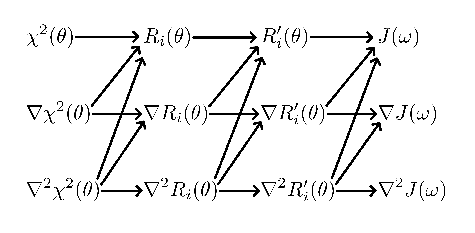
\includegraphics[width=0.8\textwidth, bb=14 14 226 110]{images/dependencies.eps.gz}}
\caption[$\chi^2$ dependencies of the values, gradients, and Hessians]{Dependencies between the $\chi^2$, transformed relaxation, relaxation, and spectral density equations, gradients, and Hessians.}\label{fig: dependencies}
\end{figure}



% Chi-squared values, gradients, and Hessians.
%%%%%%%%%%%%%%%%%%%%%%%%%%%%%%%%%%%%%%%%%%%%%%

\section{$\chi^2$ values, gradients, and Hessians}

% Chi-squared values.
\subsection{$\chi^2$ values}

The $\chi^2$ value is
\begin{equation}
 \chi^2(\theta) = \sum_{i=1}^n \frac{(\Ri - \Ri(\theta))^2}{\sigma_i^2},
\end{equation}

\noindent which is the same as equation~\eqref{eq: chi-squared} on page~\pageref{eq: chi-squared}.


% Chi-squared gradients.
\subsection{$\chi^2$ gradients}

The $\chi^2$ gradient is
\begin{equation}
 \nabla \chi^2(\theta) = 2 \sum_{i=1}^n \frac{(\Ri - \Ri(\theta))^2}{\sigma_i^2} \nabla \Ri(\theta).
\end{equation}


% Chi-squared Hessians.
\subsection{$\chi^2$ Hessians}

The $\chi^2$ Hessian is
\begin{equation}
 \nabla^2 \chi^2(\theta) = 2 \sum_{i=1}^n \frac{1}{\sigma_i^2} \left(\nabla \Ri(\theta) \cdot \nabla \Ri(\theta)^T - (\Ri - \Ri(\theta)) \nabla^2 \Ri(\theta) \right).
\end{equation}



% Ri values, gradients, and Hessians.
%%%%%%%%%%%%%%%%%%%%%%%%%%%%%%%%%%%%%

\section{$\Ri(\theta)$ values, gradients, and Hessians}


% Ri values.
\subsection{$\Ri(\theta)$ values}

The $\Ri(\theta)$ values are given by
\begin{align}
    \Rone(\theta) & = \Rone'(\theta), \label{eq: Ri trans: R1} \\
    \Rtwo(\theta) & = \Rtwo'(\theta), \label{eq: Ri trans: R2} \\
    \mathrm{NOE}(\theta) & = 1 + \frac{\gH}{\gX} \frac{\crossrate(\theta)}{\Rone(\theta)}. \label{eq: Ri trans: NOE}
\end{align}


% Ri gradients.
\subsection{$\Ri(\theta)$ gradients}

The $\Ri(\theta)$ gradients are
\begin{align}
    \nabla \Rone(\theta) & = \nabla \Rone'(\theta), \label{eq: Ri trans: dR1} \\
    \nabla \Rtwo(\theta) & = \nabla \Rtwo'(\theta), \label{eq: Ri trans: dR2} \\
    \nabla \mathrm{NOE}(\theta) & = \frac{\gH}{\gX} \frac{1}{\Rone(\theta)^2} \Big(
        \Rone(\theta) \nabla \crossrate(\theta) - \crossrate(\theta) \nabla \Rone(\theta)
    \Big). \label{eq: Ri trans: dNOE}
\end{align}


% Ri Hessians.
\subsection{$\Ri(\theta)$ Hessians}

The $\Ri(\theta)$ Hessians are
\begin{align}
    \nabla^2 \Rone(\theta) & = \nabla^2 \Rone'(\theta), \label{eq: Ri trans: d2R1} \\
    \nabla^2 \Rtwo(\theta) & = \nabla^2 \Rtwo'(\theta), \label{eq: Ri trans: d2R2} \\
    \nabla^2 \mathrm{NOE}(\theta) & = \frac{\gH}{\gX} \frac{1}{\Rone(\theta)^3} \bigg[
        \crossrate(\theta) \Big( 2 \nabla \Rone(\theta) \cdot \nabla \Rone(\theta)^T - \Rone(\theta) \nabla^2 \Rone(\theta) \Big) \nonumber\\
        & \quad - \Rone(\theta) \Big( \nabla \crossrate(\theta) \cdot \nabla \Rone(\theta)^T - \Rone(\theta) \nabla^2 \crossrate(\theta) \Big)
    \bigg]. \label{eq: Ri trans: d2NOE}
\end{align}



% Ri' values, gradients, and Hessians.
%%%%%%%%%%%%%%%%%%%%%%%%%%%%%%%%%%%%%%

\section{$\Ri'(\theta)$ values, gradients, and Hessians}

The partial and second partial derivatives of the transformed relaxation equations, $\Ri'(\theta)$, are different for each parameter of the vector $\theta$.  The vector representation of the gradient, $\nabla \textrm{R}_i'(\theta)$, and the matrix representation of the Hessian, $\nabla^2 \textrm{R}_i'(\theta)$, can be reconstructed from the individual elements presented below.


% Components
%~~~~~~~~~~~

\subsection{Components of the $\Ri'(\theta)$ equations}

To simplify the calculations of the gradients and Hessians, the $\Ri'(\theta)$ equations have been broken down into their various components.  These include the dipolar and CSA constants as well as the dipolar and CSA spectral density terms for each of the three transformed relaxation data types, $\Rone$, $\Rtwo$, and $\crossrate$.  The segregation of these components simplifies the maths as many partial derivatives of the components are zero.


% Dipolar comps.
\subsubsection{Dipolar constant}

The dipolar constant is defined as
\begin{equation}
    d = \frac{1}{4} \left(\frac{\mu_0}{4\pi}\right)^2 \frac{\left( \gH \gX \hbar \right)^2}{<r^6>}. \label{eq: Ri': d}
\end{equation}

\noindent This component of the relaxation equations is independent of the parameter of the spectral density function, $\theta_j$, the chemical exchange parameter, $\sigma_{ex}$, and the CSA parameter, $\Delta\sigma$.  Therefore, the partial and second partial derivatives with respect to these parameters is zero.  Only the partial derivative with respect to the bond length, $r$, is non-zero, being
\begin{equation}
    d' \equiv \frac{\mathrm{d} d}{\mathrm{d} r} = - \frac{3}{2} \left(\frac{\mu_0}{4\pi}\right)^2 \frac{\left( \gH \gX \hbar \right)^2}{<r^7>}. \label{eq: Ri': d'}
\end{equation}

\noindent The double partial derivative with respect to the bond length twice is
\begin{equation}
    d'' \equiv \frac{\mathrm{d}^2 d}{\mathrm{d} r^2} = \frac{21}{2} \left(\frac{\mu_0}{4\pi}\right)^2 \frac{\left( \gH \gX \hbar \right)^2}{<r^8>}. \label{eq: Ri': d"}
\end{equation}


% CSA comps.
\subsubsection{CSA constant}

The CSA constant is defined as
\begin{equation}
    c = \frac{\left(\omega_X \cdot \Delta\sigma \right)^2}{3}. \label{eq: Ri': c}
\end{equation}

\noindent The partial derivative of this component with respect to all parameters but the CSA parameter $\Delta\sigma$ is zero.  This partial derivative is
\begin{equation}
    c' \equiv \frac{\mathrm{d} c}{\mathrm{d} \Delta\sigma} = \frac{2 \omega_X^2 \cdot \Delta\sigma}{3}. \label{eq: Ri': c'}
\end{equation}

\noindent The CSA constant double partial derivative with respect to $\Delta\sigma$ is
\begin{equation}
    c'' \equiv \frac{\mathrm{d}^2 c}{\mathrm{d} \Delta\sigma^2} = \frac{2 \omega_X^2}{3}. \label{eq: Ri': c"}
\end{equation}


% R1 dip Spectral density terms.
\subsubsection{Spectral density terms of the $\Rone$ dipolar component}

For the dipolar component of the $\Rone$ equation, the spectral density terms are
\begin{equation}
    J_d^{\Rone} = J(\omega_H - \omega_X) + 3J(\omega_X) + 6J(\omega_H + \omega_X).  \label{eq: J terms: JR1d}
\end{equation}

\noindent The partial derivative of these terms with respect to the parameter of the spectral density function $\theta_j$ is
\begin{equation}
    {J_d^{\Rone}}' \equiv \frac{\partial J_d^{\Rone}}{\partial \theta_j}
        = \frac{\partial J(\omega_H - \omega_X)}{\partial \theta_j}
        + 3 \frac{\partial J(\omega_X)}{\partial \theta_j}
        + 6 \frac{\partial J(\omega_H + \omega_X)}{\partial \theta_j}.  \label{eq: J terms: JR1d'}
\end{equation}

\noindent The second partial derivative with respect to the parameter of the spectral density function $\theta_j$ and $\theta_k$ is
\begin{equation}
    {J_d^{\Rone}}'' \equiv \frac{\partial^2 J_d^{\Rone}}{\partial \theta_j \cdot \partial \theta_k}
        = \frac{\partial^2 J(\omega_H - \omega_X)}{\partial \theta_j \cdot \partial \theta_k}
        + 3 \frac{\partial^2 J(\omega_X)}{\partial \theta_j \cdot \partial \theta_k}
        + 6 \frac{\partial^2 J(\omega_H + \omega_X)}{\partial \theta_j \cdot \partial \theta_k}.  \label{eq: J terms: JR1d"}
\end{equation}


% R1 CSA Spectral density terms.
\subsubsection{Spectral density terms of the $\Rone$ CSA component}

For the CSA component of the $\Rone$ equation, the spectral density terms are
\begin{equation}
    J_c^{\Rone} = J(\omega_X).  \label{eq: J terms: JR1c}
\end{equation}

\noindent The partial derivative of these terms with respect to the parameter of the spectral density function $\theta_j$ is
\begin{equation}
    {J_c^{\Rone}}' \equiv \frac{\partial J_c^{\Rone}}{\partial \theta_j}
        = \frac{\partial J(\omega_X)}{\partial \theta_j}.  \label{eq: J terms: JR1c'}
\end{equation}

\noindent The second partial derivative with respect to the parameter of the spectral density function $\theta_j$ and $\theta_k$ is
\begin{equation}
    {J_c^{\Rone}}'' \equiv \frac{\partial^2 J_c^{\Rone}}{\partial \theta_j . \partial \theta_k}
        = \frac{\partial^2 J(\omega_X)}{\partial \theta_j \cdot \partial \theta_k}.  \label{eq: J terms: JR1c"}
\end{equation}


% R2 dip Spectral density terms.
\subsubsection{Spectral density terms of the $\Rtwo$ dipolar component}

For the dipolar component of the $\Rtwo$ equation, the spectral density terms are
\begin{equation}
    J_d^{\Rtwo} = 4J(0) + J(\omega_H - \omega_X) + 3J(\omega_X) + 6J(\omega_H) + 6J(\omega_H + \omega_X).  \label{eq: J terms: JR2d}
\end{equation}

\noindent The partial derivative of these terms with respect to the parameter of the spectral density function $\theta_j$ is
\begin{equation}
    {J_d^{\Rtwo}}' \equiv \frac{\partial J_d^{\Rtwo}}{\partial \theta_j}
        = 4 \frac{\partial J(0)}{\partial \theta_j}
        + \frac{\partial J(\omega_H - \omega_X)}{\partial \theta_j}
        + 3 \frac{\partial J(\omega_X)}{\partial \theta_j}
        + 6 \frac{\partial J(\omega_H)}{\partial \theta_j}
        + 6 \frac{\partial J(\omega_H + \omega_X)}{\partial \theta_j}.  \label{eq: J terms: JR2d'}
\end{equation}

\noindent The second partial derivative with respect to the parameter of the spectral density function $\theta_j$ and $\theta_k$ is
\begin{multline}
    {J_d^{\Rtwo}}'' \equiv \frac{\partial^2 J_d^{\Rtwo}}{\partial \theta_j \cdot \partial \theta_k}
        = 4 \frac{\partial^2 J(0)}{\partial \theta_j \cdot \partial \theta_k}
        + \frac{\partial^2 J(\omega_H - \omega_X)}{\partial \theta_j \cdot \partial \theta_k}
        + 3 \frac{\partial^2 J(\omega_X)}{\partial \theta_j \cdot \partial \theta_k} \\
        + 6 \frac{\partial^2 J(\omega_H)}{\partial \theta_j \cdot \partial \theta_k}
        + 6 \frac{\partial^2 J(\omega_H + \omega_X)}{\partial \theta_j \cdot \partial \theta_k}.  \label{eq: J terms: JR2d"}
\end{multline}


% R2 CSA Spectral density terms.
\subsubsection{Spectral density terms of the $\Rtwo$ CSA component}

For the CSA component of the $\Rtwo$ equation, the spectral density terms are
\begin{equation}
    J_c^{\Rtwo} = 4J(0) + 3J(\omega_X).  \label{eq: J terms: JR2c}
\end{equation}

\noindent The partial derivative of these terms with respect to the parameter of the spectral density function $\theta_j$ is
\begin{equation}
    {J_c^{\Rtwo}}' \equiv \frac{\partial J_c^{\Rtwo}}{\partial \theta_j}
        = 4 \frac{\partial J(0)}{\partial \theta_j}
        + 3 \frac{\partial J(\omega_X)}{\partial \theta_j}.  \label{eq: J terms: JR2c'}
\end{equation}

\noindent The second partial derivative with respect to the parameter of the spectral density function $\theta_j$ and $\theta_k$ is
\begin{equation}
    {J_c^{\Rtwo}}'' \equiv \frac{\partial^2 J_c^{\Rtwo}}{\partial \theta_j \cdot \partial \theta_k}
        = 4 \frac{\partial^2 J(0)}{\partial \theta_j \cdot \partial \theta_k}
        + 3 \frac{\partial^2 J(\omega_X)}{\partial \theta_j \cdot \partial \theta_k}.  \label{eq: J terms: JR2c"}
\end{equation}


% Sigma_NOE dip Spectral density terms.
\subsubsection{Spectral density terms of the $\crossrate$ dipolar component}

For the dipolar component of the $\crossrate$ equation, the spectral density terms are
\begin{equation}
    J_d^{\crossrate} = 6J(\omega_H + \omega_X) - 6J(\omega_H - \omega_X).  \label{eq: J terms: JsigmaNOEd}
\end{equation}

\noindent The partial derivative of these terms with respect to the parameter of the spectral density function $\theta_j$ is
\begin{equation}
    {J_d^{\crossrate}}' \equiv \frac{\partial J_d^{\crossrate}}{\partial \theta_j}
        = 6 \frac{\partial J(\omega_H + \omega_X)}{\partial \theta_j}
        - 6 \frac{\partial J(\omega_H - \omega_X)}{\partial \theta_j}.  \label{eq: J terms: JsigmaNOEd'}
\end{equation}

\noindent The second partial derivative with respect to the parameter of the spectral density function $\theta_j$ and $\theta_k$ is
\begin{equation}
    {J_d^{\crossrate}}'' \equiv \frac{\partial^2 J_d^{\crossrate}}{\partial \theta_j \cdot \partial \theta_k}
        = 6 \frac{\partial^2 J(\omega_H + \omega_X)}{\partial \theta_j \cdot \partial \theta_k}
        - 6 \frac{\partial^2 J(\omega_H - \omega_X)}{\partial \theta_j \cdot \partial \theta_k}.  \label{eq: J terms: JsigmaNOEd"}
\end{equation}



% Ri' values.
%~~~~~~~~~~~~~~~

\subsection{$\Ri'(\theta)$ values}

The three relaxation equations, utilising the above components, can be expressed as
\begin{align}
    \Rone(\theta) & = d J_d^{\Rone} + c J_c^{\Rone},                          \label{eq: Ri': R1} \\
    \Rtwo(\theta) & = \frac{d}{2} J_d^{\Rtwo} + \frac{c}{6} J_c^{\Rtwo},      \label{eq: Ri': R2} \\
    \crossrate(\theta) & = d J_d^{\crossrate}.                          \label{eq: Ri': sigmaNOE}
\end{align}



% Ri' gradients.
%~~~~~~~~~~~~~~~

\subsection{$\Ri'(\theta)$ gradients}

The partial derivatives with respect to the parameter of the spectral density functions, the chemical exchange parameter, CSA parameter, and bond length parameters are all different and are presented below.


% Spectral density function parameter.
\subsubsection{Spectral density function parameter}

The partial derivatives of the relaxation equations with respect to the parameter of the spectral density function $\theta_j$ are
\begin{align}
    \frac{\partial \Rone(\theta)}{\partial \theta_j} &= d {J_d^{\Rone}}' + c {J_c^{\Rone}}',                      \label{eq: Ri': dR1/dmf} \\
    \frac{\partial \Rtwo(\theta)}{\partial \theta_j} &= \frac{d}{2} {J_d^{\Rtwo}}' + \frac{c}{6} {J_c^{\Rtwo}}',  \label{eq: Ri': dR2/dmf} \\
    \frac{\partial \crossrate(\theta)}{\partial \theta_j} &= d {J_d^{\crossrate}}'.                         \label{eq: Ri': dsigmaNOE/dmf}
\end{align}


% Chemical exchange parameter.
\subsubsection{Chemical exchange parameter}

The partial derivatives of the relaxation equations with respect to the chemical exchange parameter $R_{ex}$ are
\begin{align}
    \frac{\partial \Rone(\theta)}{\partial R_{ex}} &= 0,          \label{eq: Ri': dR1/dRex} \\
    \frac{\partial \Rtwo(\theta)}{\partial R_{ex}} &= 1,          \label{eq: Ri': dR2/dRex} \\
    \frac{\partial \crossrate(\theta)}{\partial R_{ex}} &= 0.   \label{eq: Ri': dsigmaNOE/dRex}
\end{align}


% CSA parameter.
\subsubsection{CSA parameter}

The partial derivatives of the relaxation equations with respect to the CSA parameter $\Delta\sigma$ are
\begin{align}
    \frac{\partial \Rone(\theta)}{\partial \Delta\sigma} &= c' J_c^{\Rone},             \label{eq: Ri': dR1/dCSA} \\
    \frac{\partial \Rtwo(\theta)}{\partial \Delta\sigma} &= \frac{c'}{6} J_c^{\Rtwo},   \label{eq: Ri': dR2/dCSA} \\
    \frac{\partial \crossrate(\theta)}{\partial \Delta\sigma} &= 0.                 \label{eq: Ri': dsigmaNOE/dCSA}
\end{align}


% Bond length parameter.
\subsubsection{Bond length parameter}

The partial derivatives of the relaxation equations with respect to the bond length parameter $r$ are
\begin{align}
    \frac{\partial \Rone(\theta)}{\partial r} &= d' J_d^{\Rone},                \label{eq: Ri': dR1/dr} \\
    \frac{\partial \Rtwo(\theta)}{\partial r} &= \frac{d'}{2} J_d^{\Rtwo},      \label{eq: Ri': dR2/dr} \\
    \frac{\partial \crossrate(\theta)}{\partial r} &= d' J_d^{\crossrate}.  \label{eq: Ri': dsigmaNOE/dr}
\end{align}


% Ri' Hessians.
%~~~~~~~~~~~~~~

\subsection{$\Ri'(\theta)$ Hessians}

The second partial derivatives with respect to the parameter of the spectral density functions, the chemical exchange parameter, CSA parameter, and bond length parameters are presented below.


% Spectral density function parameter - Spectral density function parameter.
\subsubsection{Spectral density function parameter - Spectral density function parameter}

The second partial derivatives of the relaxation equations with respect to the parameter of the spectral density functions $\theta_j$ and $\theta_k$ are
\begin{align}
    \frac{\partial^2 \Rone(\theta)}{\partial \theta_j \cdot \partial \theta_k} &= d {J_d^{\Rone}}'' + c {J_c^{\Rone}}'',                      \label{eq: Ri': d2R1/dmfj.dmfk} \\
    \frac{\partial^2 \Rtwo(\theta)}{\partial \theta_j \cdot \partial \theta_k} &= \frac{d}{2} {J_d^{\Rtwo}}'' + \frac{c}{6} {J_c^{\Rtwo}}'',  \label{eq: Ri': d2R2/dmfj.dmfk} \\
    \frac{\partial^2 \crossrate(\theta)}{\partial \theta_j \cdot \partial \theta_k} &= d {J_d^{\crossrate}}''.                          \label{eq: Ri': d2sigmaNOE/dmfj.dmfk}
\end{align}


% Spectral density function parameter - Chemical exchange parameter.
\subsubsection{Spectral density function parameter - Chemical exchange parameter}

The second partial derivatives of the relaxation equations with respect to the parameter of the spectral density function $\theta_j$ and the chemical exchange parameter $R_{ex}$ are
\begin{align}
    \frac{\partial^2 \Rone(\theta)}{\partial \theta_j \cdot \partial R_{ex}} &= 0,        \label{eq: Ri': d2R1/dmfj.dRex} \\
    \frac{\partial^2 \Rtwo(\theta)}{\partial \theta_j \cdot \partial R_{ex}} &= 0,        \label{eq: Ri': d2R2/dmfj.dRex} \\
    \frac{\partial^2 \crossrate(\theta)}{\partial \theta_j \cdot \partial R_{ex}} &= 0. \label{eq: Ri': d2sigmaNOE/dmfj.dRex}
\end{align}


% Spectral density function parameter - CSA parameter.
\subsubsection{Spectral density function parameter - CSA parameter}

The second partial derivatives of the relaxation equations with respect to the parameter of the spectral density function $\theta_j$ and the CSA parameter $\Delta\sigma$ are
\begin{align}
    \frac{\partial^2 \Rone(\theta)}{\partial \theta_j \cdot \partial \Delta\sigma} &= c' {J_c^{\Rone}}',            \label{eq: Ri': d2R1/dmfj.dCSA} \\
    \frac{\partial^2 \Rtwo(\theta)}{\partial \theta_j \cdot \partial \Delta\sigma} &= \frac{c'}{6} {J_c^{\Rtwo}}',  \label{eq: Ri': d2R2/dmfj.dCSA} \\
    \frac{\partial^2 \crossrate(\theta)}{\partial \theta_j \cdot \partial \Delta\sigma} &= 0.                   \label{eq: Ri': d2sigmaNOE/dmfj.dCSA}
\end{align}


% Spectral density function parameter - Bond length parameter.
\subsubsection{Spectral density function parameter - Bond length parameter}

The second partial derivatives of the relaxation equations with respect to the parameter of the spectral density function $\theta_j$ and the bond length parameter $r$ are
\begin{align}
    \frac{\partial^2 \Rone(\theta)}{\partial \theta_j \cdot \partial r} &= d' {J_d^{\Rone}}',               \label{eq: Ri': d2R1/dmfj.dr} \\
    \frac{\partial^2 \Rtwo(\theta)}{\partial \theta_j \cdot \partial r} &= \frac{d'}{2} {J_d^{\Rtwo}}',     \label{eq: Ri': d2R2/dmfj.dr} \\
    \frac{\partial^2 \crossrate(\theta)}{\partial \theta_j \cdot \partial r} &= d' {J_d^{\crossrate}}'. \label{eq: Ri': d2sigmaNOE/dmfj.dr}
\end{align}


% Chemical exchange parameter - Chemical exchange parameter.
\subsubsection{Chemical exchange parameter - Chemical exchange parameter}

The second partial derivatives of the relaxation equations with respect to the chemical exchange parameter $R_{ex}$ twice are
\begin{align}
    \frac{\partial^2 \Rone(\theta)}{{\partial R_{ex}}^2} &= 0,        \label{eq: Ri': d2R1/dRex2} \\
    \frac{\partial^2 \Rtwo(\theta)}{{\partial R_{ex}}^2} &= 0,        \label{eq: Ri': d2R2/dRex2} \\
    \frac{\partial^2 \crossrate(\theta)}{{\partial R_{ex}}^2} &= 0. \label{eq: Ri': d2sigmaNOE/dRex2}
\end{align}


% Chemical exchange parameter - CSA parameter.
\subsubsection{Chemical exchange parameter - CSA parameter}

The second partial derivatives of the relaxation equations with respect to the chemical exchange parameter $R_{ex}$ and the CSA parameter $\Delta\sigma$ are
\begin{align}
    \frac{\partial^2 \Rone(\theta)}{\partial R_{ex} \cdot \partial \Delta\sigma} &= 0,        \label{eq: Ri': d2R1/dRex.dCSA} \\
    \frac{\partial^2 \Rtwo(\theta)}{\partial R_{ex} \cdot \partial \Delta\sigma} &= 0,        \label{eq: Ri': d2R2/dRex.dCSA} \\
    \frac{\partial^2 \crossrate(\theta)}{\partial R_{ex} \cdot \partial \Delta\sigma} &= 0. \label{eq: Ri': d2sigmaNOE/dRex.dCSA}
\end{align}


% Chemical exchange parameter - Bond length parameter.
\subsubsection{Chemical exchange parameter - Bond length parameter}

The second partial derivatives of the relaxation equations with respect to the chemical exchange parameter $R_{ex}$ and the bond length parameter $r$ are
\begin{align}
    \frac{\partial^2 \Rone(\theta)}{\partial R_{ex} \cdot \partial r} &= 0,           \label{eq: Ri': d2R1/dRex.dr} \\
    \frac{\partial^2 \Rtwo(\theta)}{\partial R_{ex} \cdot \partial r} &= 0,           \label{eq: Ri': d2R2/dRex.dr} \\
    \frac{\partial^2 \crossrate(\theta)}{\partial R_{ex} \cdot \partial r} &= 0.    \label{eq: Ri': d2sigmaNOE/dRex.dr}
\end{align}


% CSA parameter - CSA parameter.
\subsubsection{CSA parameter - CSA parameter}

The second partial derivatives of the relaxation equations with respect to the CSA parameter $\Delta\sigma$ twice are
\begin{align}
    \frac{\partial^2 \Rone(\theta)}{{\partial \Delta\sigma}^2} &= c'' J_c^{\Rone},              \label{eq: Ri': d2R1/dCSA2} \\
    \frac{\partial^2 \Rtwo(\theta)}{{\partial \Delta\sigma}^2} &= \frac{c''}{6} J_c^{\Rtwo},    \label{eq: Ri': d2R2/dCSA2} \\
    \frac{\partial^2 \crossrate(\theta)}{{\partial \Delta\sigma}^2} &= 0.                   \label{eq: Ri': d2sigmaNOE/dCSA2}
\end{align}


% CSA parameter - Bond length parameter.
\subsubsection{CSA parameter - Bond length parameter}

The second partial derivatives of the relaxation equations with respect to the CSA parameter $\Delta\sigma$ and the bond length parameter $r$ are
\begin{align}
    \frac{\partial^2 \Rone(\theta)}{\partial \Delta\sigma \cdot \partial r} &= 0,         \label{eq: Ri': d2R1/dCSA.dr} \\
    \frac{\partial^2 \Rtwo(\theta)}{\partial \Delta\sigma \cdot \partial r} &= 0,         \label{eq: Ri': d2R2/dCSA.dr} \\
    \frac{\partial^2 \crossrate(\theta)}{\partial \Delta\sigma \cdot \partial r} &= 0.  \label{eq: Ri': d2sigmaNOE/dCSA.dr}
\end{align}


% Bond length parameter - Bond length parameter.
\subsubsection{Bond length parameter - Bond length parameter}

The second partial derivatives of the relaxation equations with respect to the bond length parameter $r$ twice are
\begin{align}
    \frac{\partial^2 \Rone(\theta)}{{\partial r}^2} &= d'' J_d^{\Rone},                 \label{eq: Ri': d2R1/dr2} \\
    \frac{\partial^2 \Rtwo(\theta)}{{\partial r}^2} &= \frac{d''}{2} J_d^{\Rtwo},       \label{eq: Ri': d2R2/dr2} \\
    \frac{\partial^2 \crossrate(\theta)}{{\partial r}^2} &= d'' J_d^{\crossrate}.   \label{eq: Ri': d2sigmaNOE/dr2}
\end{align}



% Ellipsoidal diffusion tensor.
%%%%%%%%%%%%%%%%%%%%%%%%%%%%%%%

\section{Ellipsoidal diffusion tensor}

\index{diffusion!ellipsoid (asymmetric)}


% Ellipsoid weight derivatives.
%~~~~~~~~~~~~~~~~~~~~~~~~~~~~~~

\subsection{Ellipsoid weight derivatives}


